% !TEX output_directory = ./build

%%%%%%%%%%%%%%%%%%%%%%%%%%%%%%%%%%%%%%%%%%%%%%%%%%%%%%%%%%%%%%%%%%%%%%%%
% Autonomous Intelligent System, University of Bonn, LaTeX Beamer theme
%
% Copyright (C) 2010-2013 Dirk Holz, dirk.holz@ieee.org

% This program is free software: you can redistribute it and/or modify
% it under the terms of the GNU General Public License as published by
% the Free Software Foundation, either version 3 of the License, or
% (at your option) any later version.

% This program is distributed in the hope that it will be useful,
% but WITHOUT ANY WARRANTY; without even the implied warranty of
% MERCHANTABILITY or FITNESS FOR A PARTICULAR PURPOSE.  See the
% GNU General Public License for more details.

% You should have received a copy of the GNU General Public License
% along with this program.  If not, see <http://www.gnu.org/licenses/>.

\documentclass[unknownkeysallowed]{beamer}
\let\Tiny=\tiny

% all available options --->
% \usetheme[shadow,logoinnavbar,subsection,logoinframe,framenavbar]{AIS}
\usetheme[shadow,logoinnavbar,subsection]{BIT}

\usepackage{listings}
\usepackage{mathtools}
\usepackage{graphicx}

\DeclarePairedDelimiter\ceil{\lceil}{\rceil}
\DeclarePairedDelimiter\floor{\lfloor}{\rfloor}

\title[Master seminar:  Solving localization problem in first person computer games with deep learning]{Master seminar:  Solving localization problem in first person computer games with deep learning}
% \subtitle{}
% \begin{minipage}{0.4\textwidth}
%   \begin{flushleft} \large
%   \emph{Author:}\\
%   Yauheni \textsc{Selivonchyk} % Your name
%   \end{flushleft}
% \end{minipage}
% ~
% \begin{minipage}{0.5\textwidth}
%   \begin{flushright} \large
%   \emph{Supervisor:} \\
%   Prof. Dr. Christian \textsc{Bauckhage} % Supervisor's Name
%
%   \end{flushright}
% \end{minipage}\\[0.5cm]
%
% \begin{minipage}{0.3\textwidth}
%   \begin{flushleft} \large
%   \end{flushleft}
% \end{minipage}
% ~
% \begin{minipage}{0.6\textwidth}
%   \begin{flushright} \large
%   \emph{Second Supervisor:} \\
%   Prof. Dr. Stefan \textsc{Wrobel} % Supervisor's Name
%
%   \end{flushright}
% \end{minipage}\\[0.5cm]

\author[Y. Selivonchyk]{\highlight{Yauheni Selivonchyk}\inst{1}, Michael Kamp\inst{2}}
\institute[University of Bonn]
{
  \inst{1}%
  Student of Master Computer Science,\\
  University of Bonn
  \and
  \inst{2}Fraunhofer Institute for Intelligent Analysis and Informations Systems IAIS
}

\begin{columns}[T] % align columns
\begin{column}{.48\textwidth}
\color{red}\rule{\linewidth}{4pt}

Left Part
\end{column}%
\hfill%
\begin{column}{.48\textwidth}
\color{blue}\rule{\linewidth}{4pt}

Right Part
\end{column}%
\end{columns}

\date{\today}

% This is only inserted into the PDF information catalog. Can be left out.
\subject{Talks}

% Delete this, if you do not want the table of contents to pop up at
% the beginning of each subsection:
\AtBeginSection[]
{
  \begin{frame}<beamer>
    \frametitle{Outline}
    \tableofcontents[currentsection,hideothersubsection]
  \end{frame}
}

% If you wish to uncover everything in a step-wise fashion, uncomment
% the following command:
% \beamerdefaultoverlayspecification{<+->}

\begin{document}
\lstset{language=Python}

\begin{frame}
  \titlepage
\end{frame}


\begin{frame}{Support vector machines}
Support vector machines generalize well given sufficient amount of training data.\\
General SVM algorithm solves next empirical risk optimization problem:
\begin{equation}\label{eq:dual}
\begin{aligned}
\max\limits_{\alpha} \sum_{i=1}^n \alpha_i -1/2 \sum_{i,j=1}^n \alpha_i\alpha_j y_i y_j  k(x_i, x_j) \\
\alpha_i > 0 , \sum_{i=1}^n\alpha_i y_i=0
\end{aligned}
\end{equation}
Where $k(x, y)$ is kernel function:
\begin{equation}\label{eq:kernel}
k(x,y)=\langle\Phi(x), \Phi(y)\rangle
\end{equation}
\end{frame}

\begin{frame}{Support vector machines. Continued}
Whenever mapping $\Phi(x)$ of $x$ into Hilbert space is explicitly known:
\begin{equation}\label{eq:kernel}
\Phi: \mathcal{X} \to \mathcal{V}
\end{equation}
and $\mathcal{V}$ is of relatively low dimension $D$.

Training and evaluation time can then be reduced from $O(n^2)$ and $O(n)$ to $O(nD)$ and $O(D)$ respectively.
\vspace{1cm}
\begin{center}
Can we find such a mapping for every function $k(x, y)$?
\end{center}
\end{frame}

\begin{frame}{Random Fourier features}
  Solution provided by Rahimi and Rechts (2007) suggests relatively low-dimensional mapping for stationary kernels:
  \begin{equation}\label{eq:stationary}
k_s(z) = k_s(x-y) = k(x, y)
\end{equation}
By Bochner theorem (1956) any positive semi-definite function as $k_s(z)$ can be expressed as:
\begin{equation}
k_s(x-y)= \int_{\mathbb{R}^d} p(\omega) cos \omega(x-y) d\omega
\end{equation}
where $p(\omega)$ is a finite measure. Therefore we can estimate $k_s(z)$ as:
\begin{equation}
k_s(x-y) = E_\omega[cos\omega(x-y)] \approx z_\omega(x)z_\omega(y)^*
\end{equation}
\end{frame}


\begin{frame}{Kernel function approximation rate}
\begin{figure}
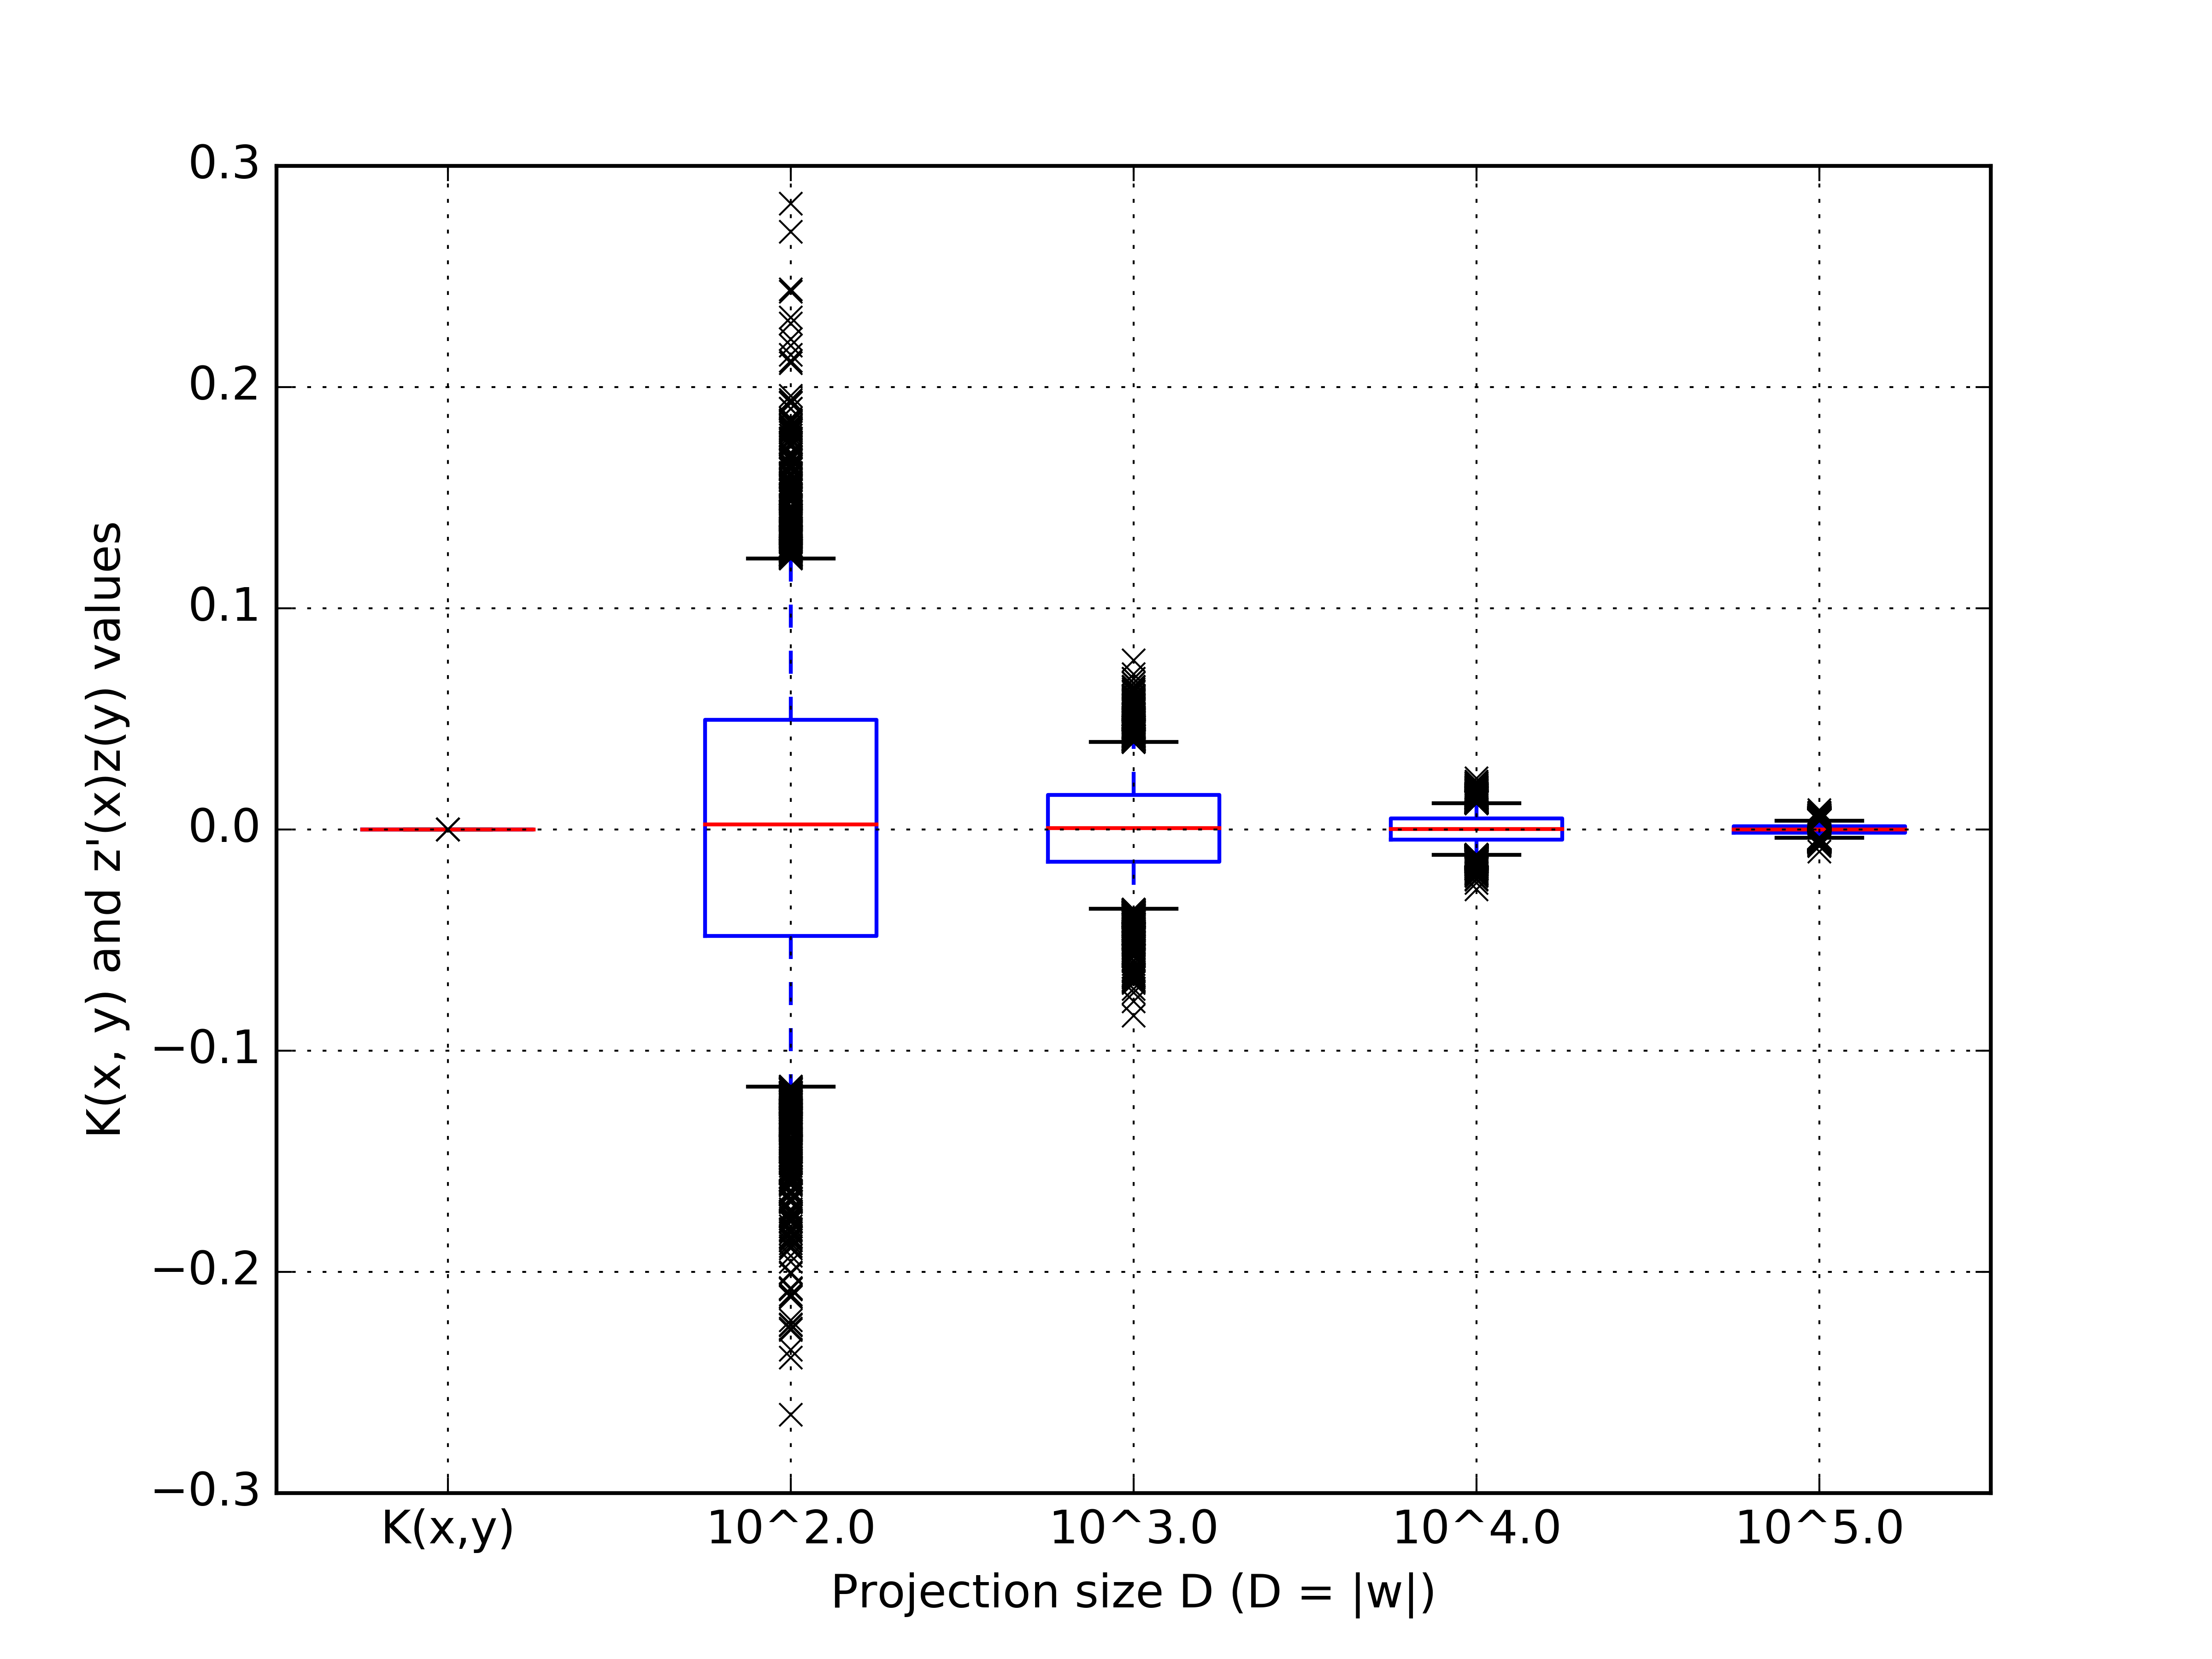
\includegraphics[scale=0.45]{img/test_precision_interval_delta_}
\end{figure}
\end{frame}

\begin{frame}{Qualities of input space}
\begin{figure}
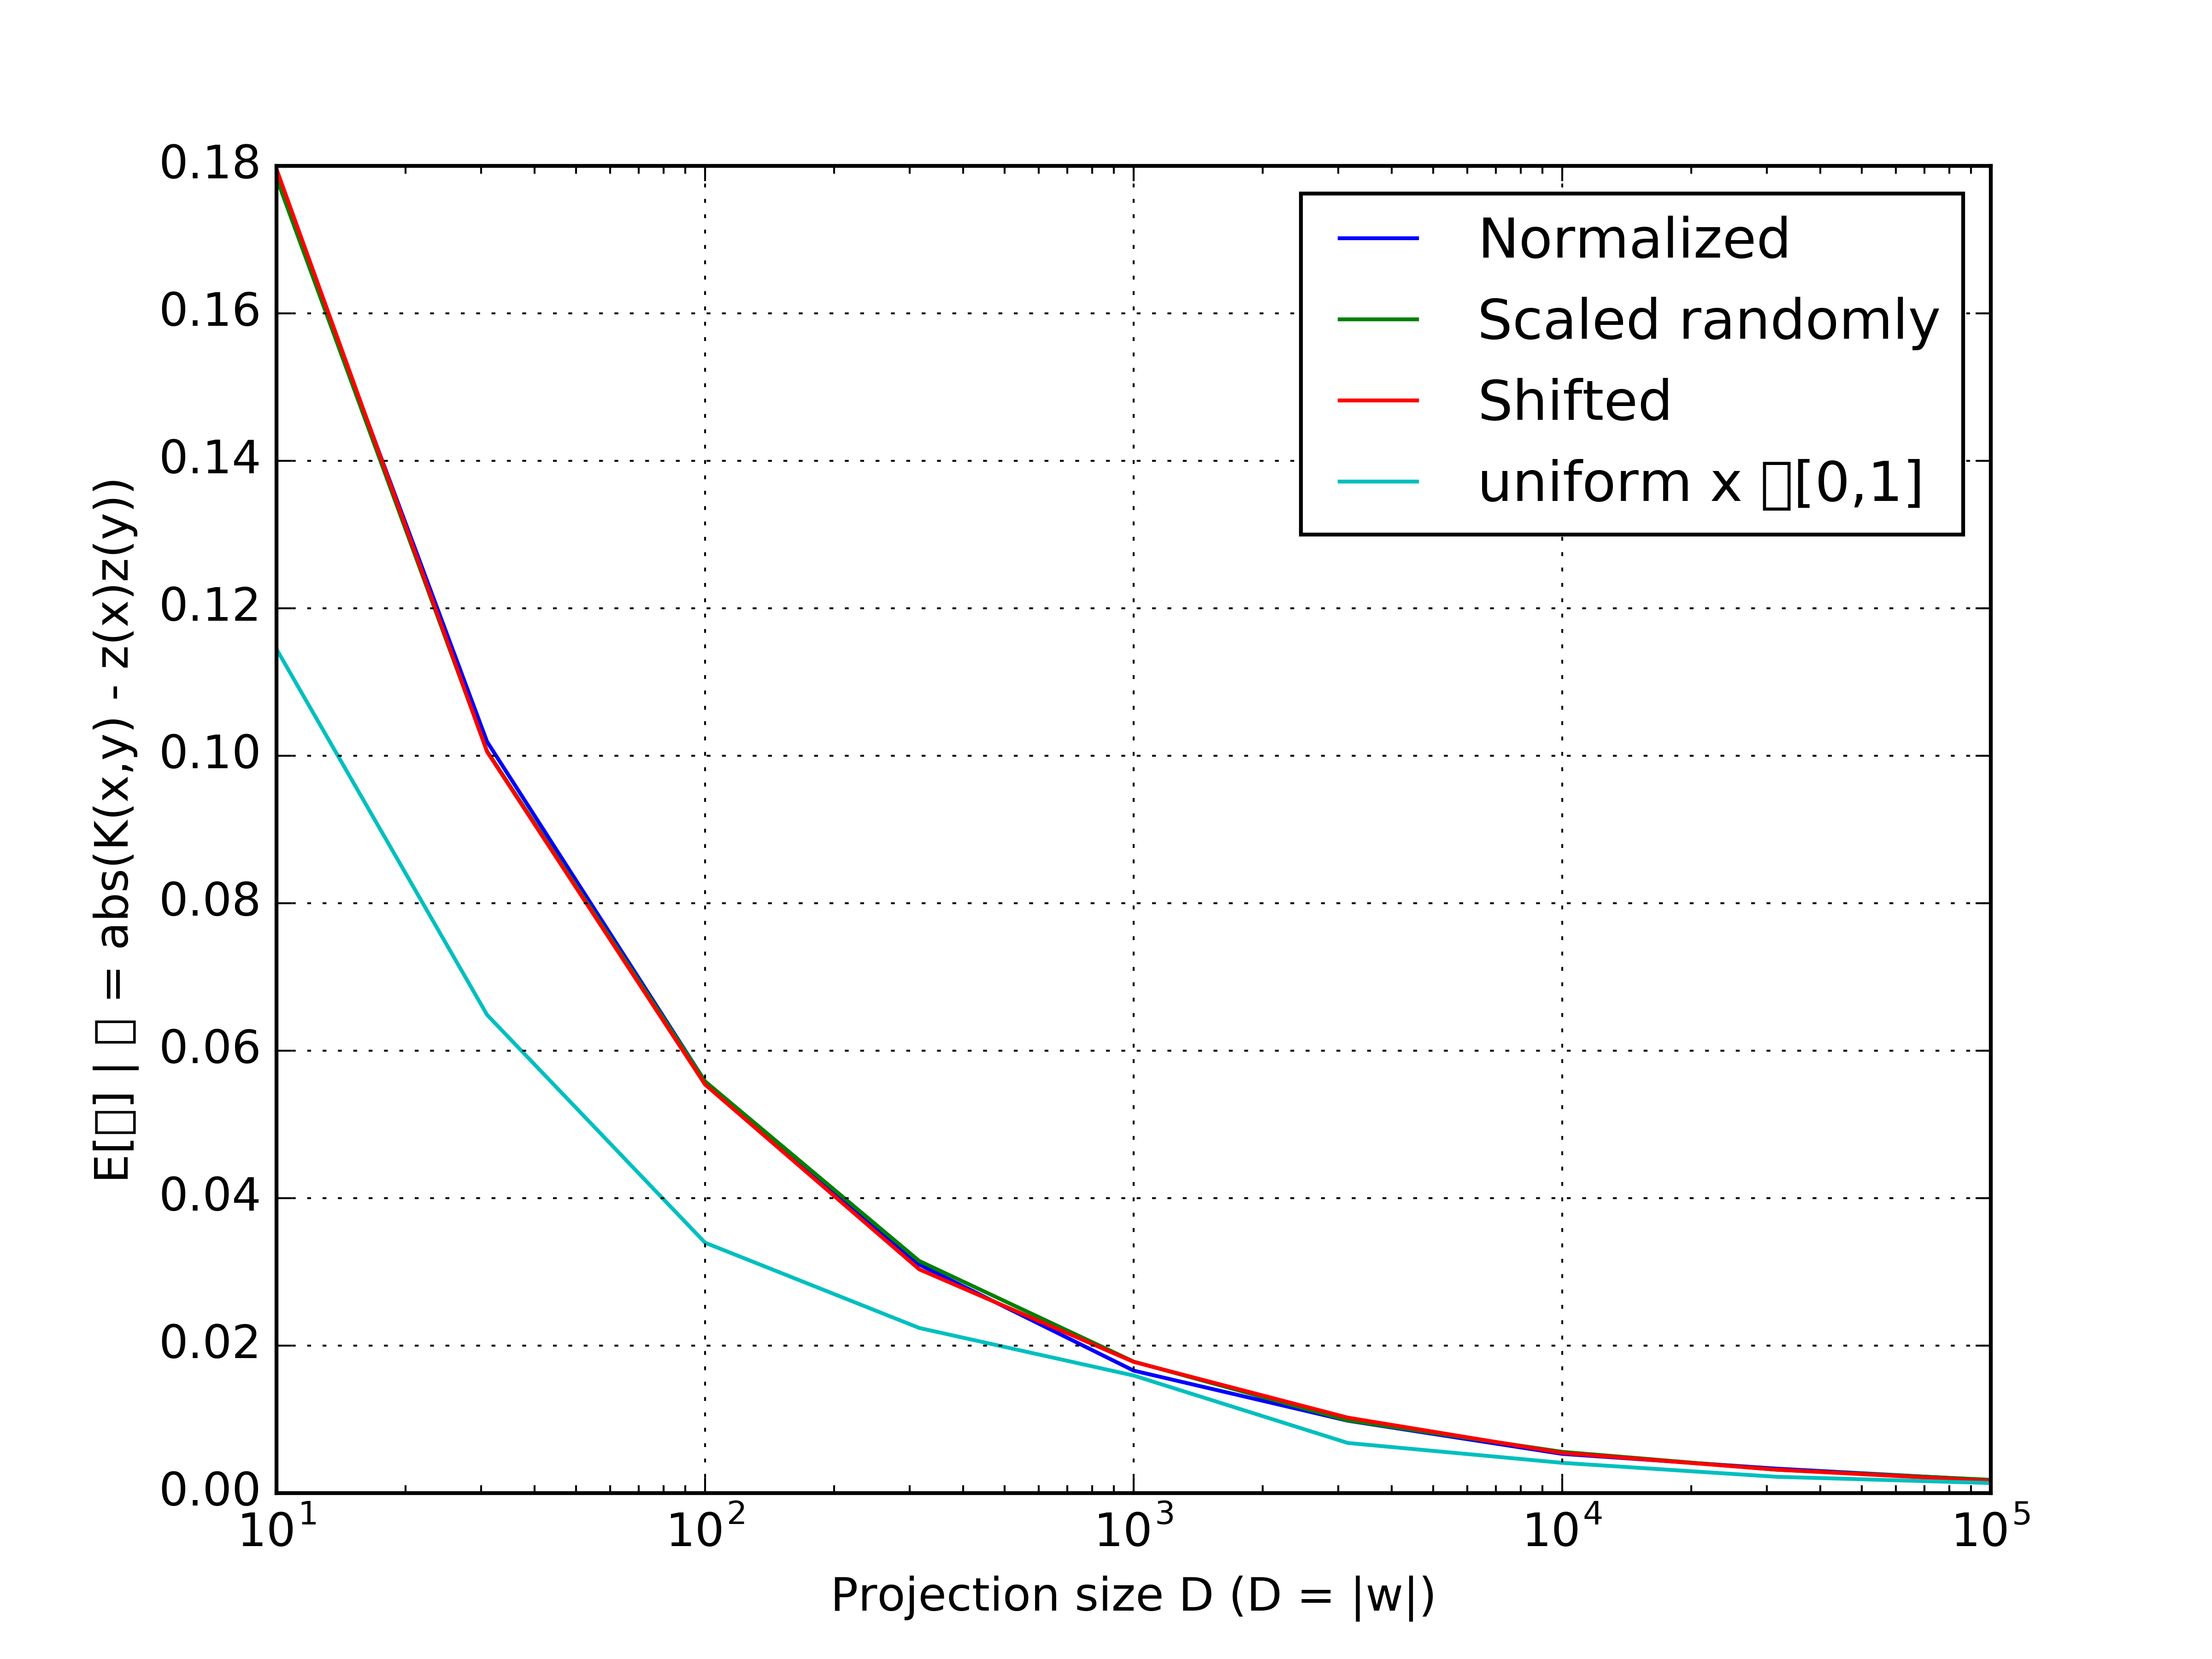
\includegraphics[scale=0.45]{img/fig_input_}
\end{figure}
\end{frame}

\begin{frame}{LinearSVM using RFF vs SVM. Input}
\begin{figure}
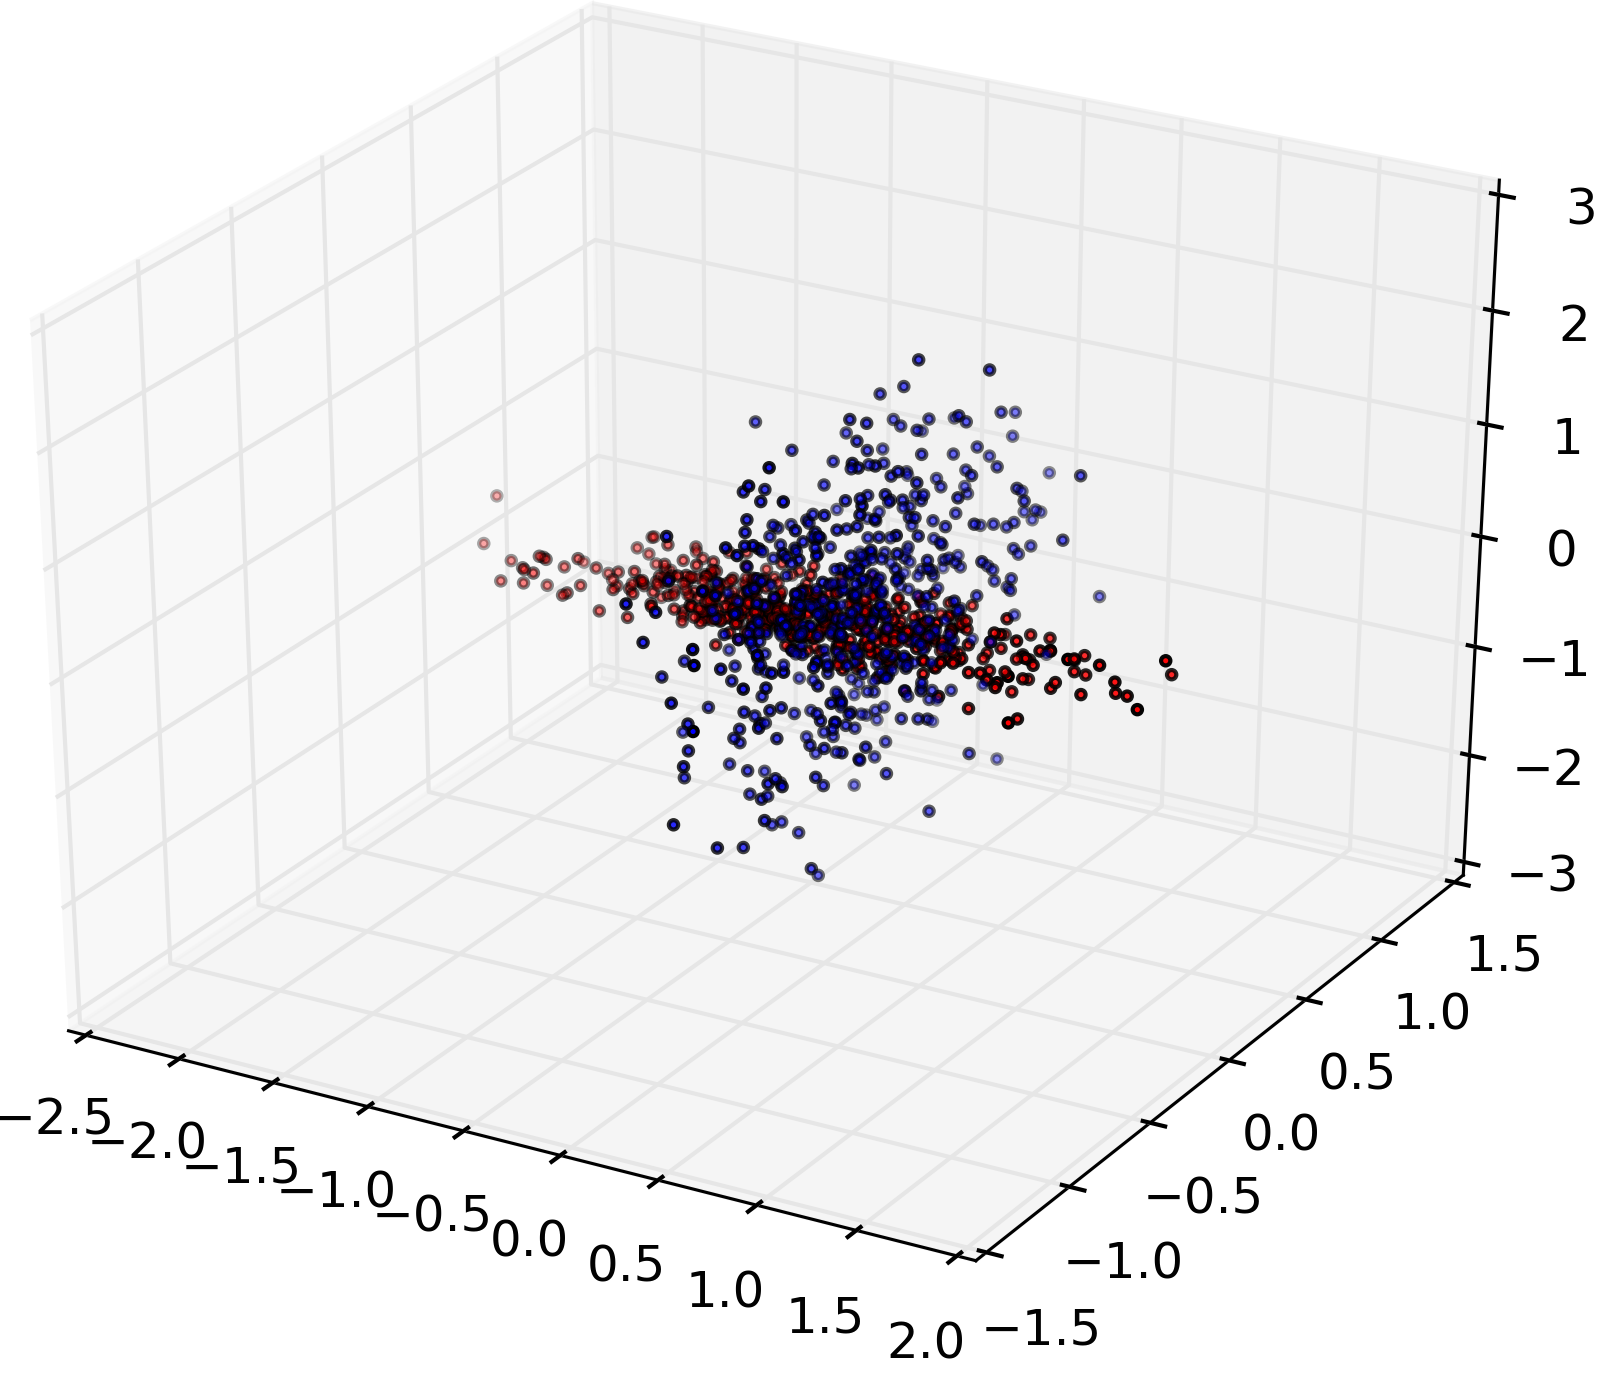
\includegraphics[scale=0.145]{img/svm_tm_n10_N131072_k10--3d_copy}
\end{figure}
\end{frame}

\begin{frame}[noframenumbering]{LinearSVM using RFF vs SVM. Input}
\begin{figure}
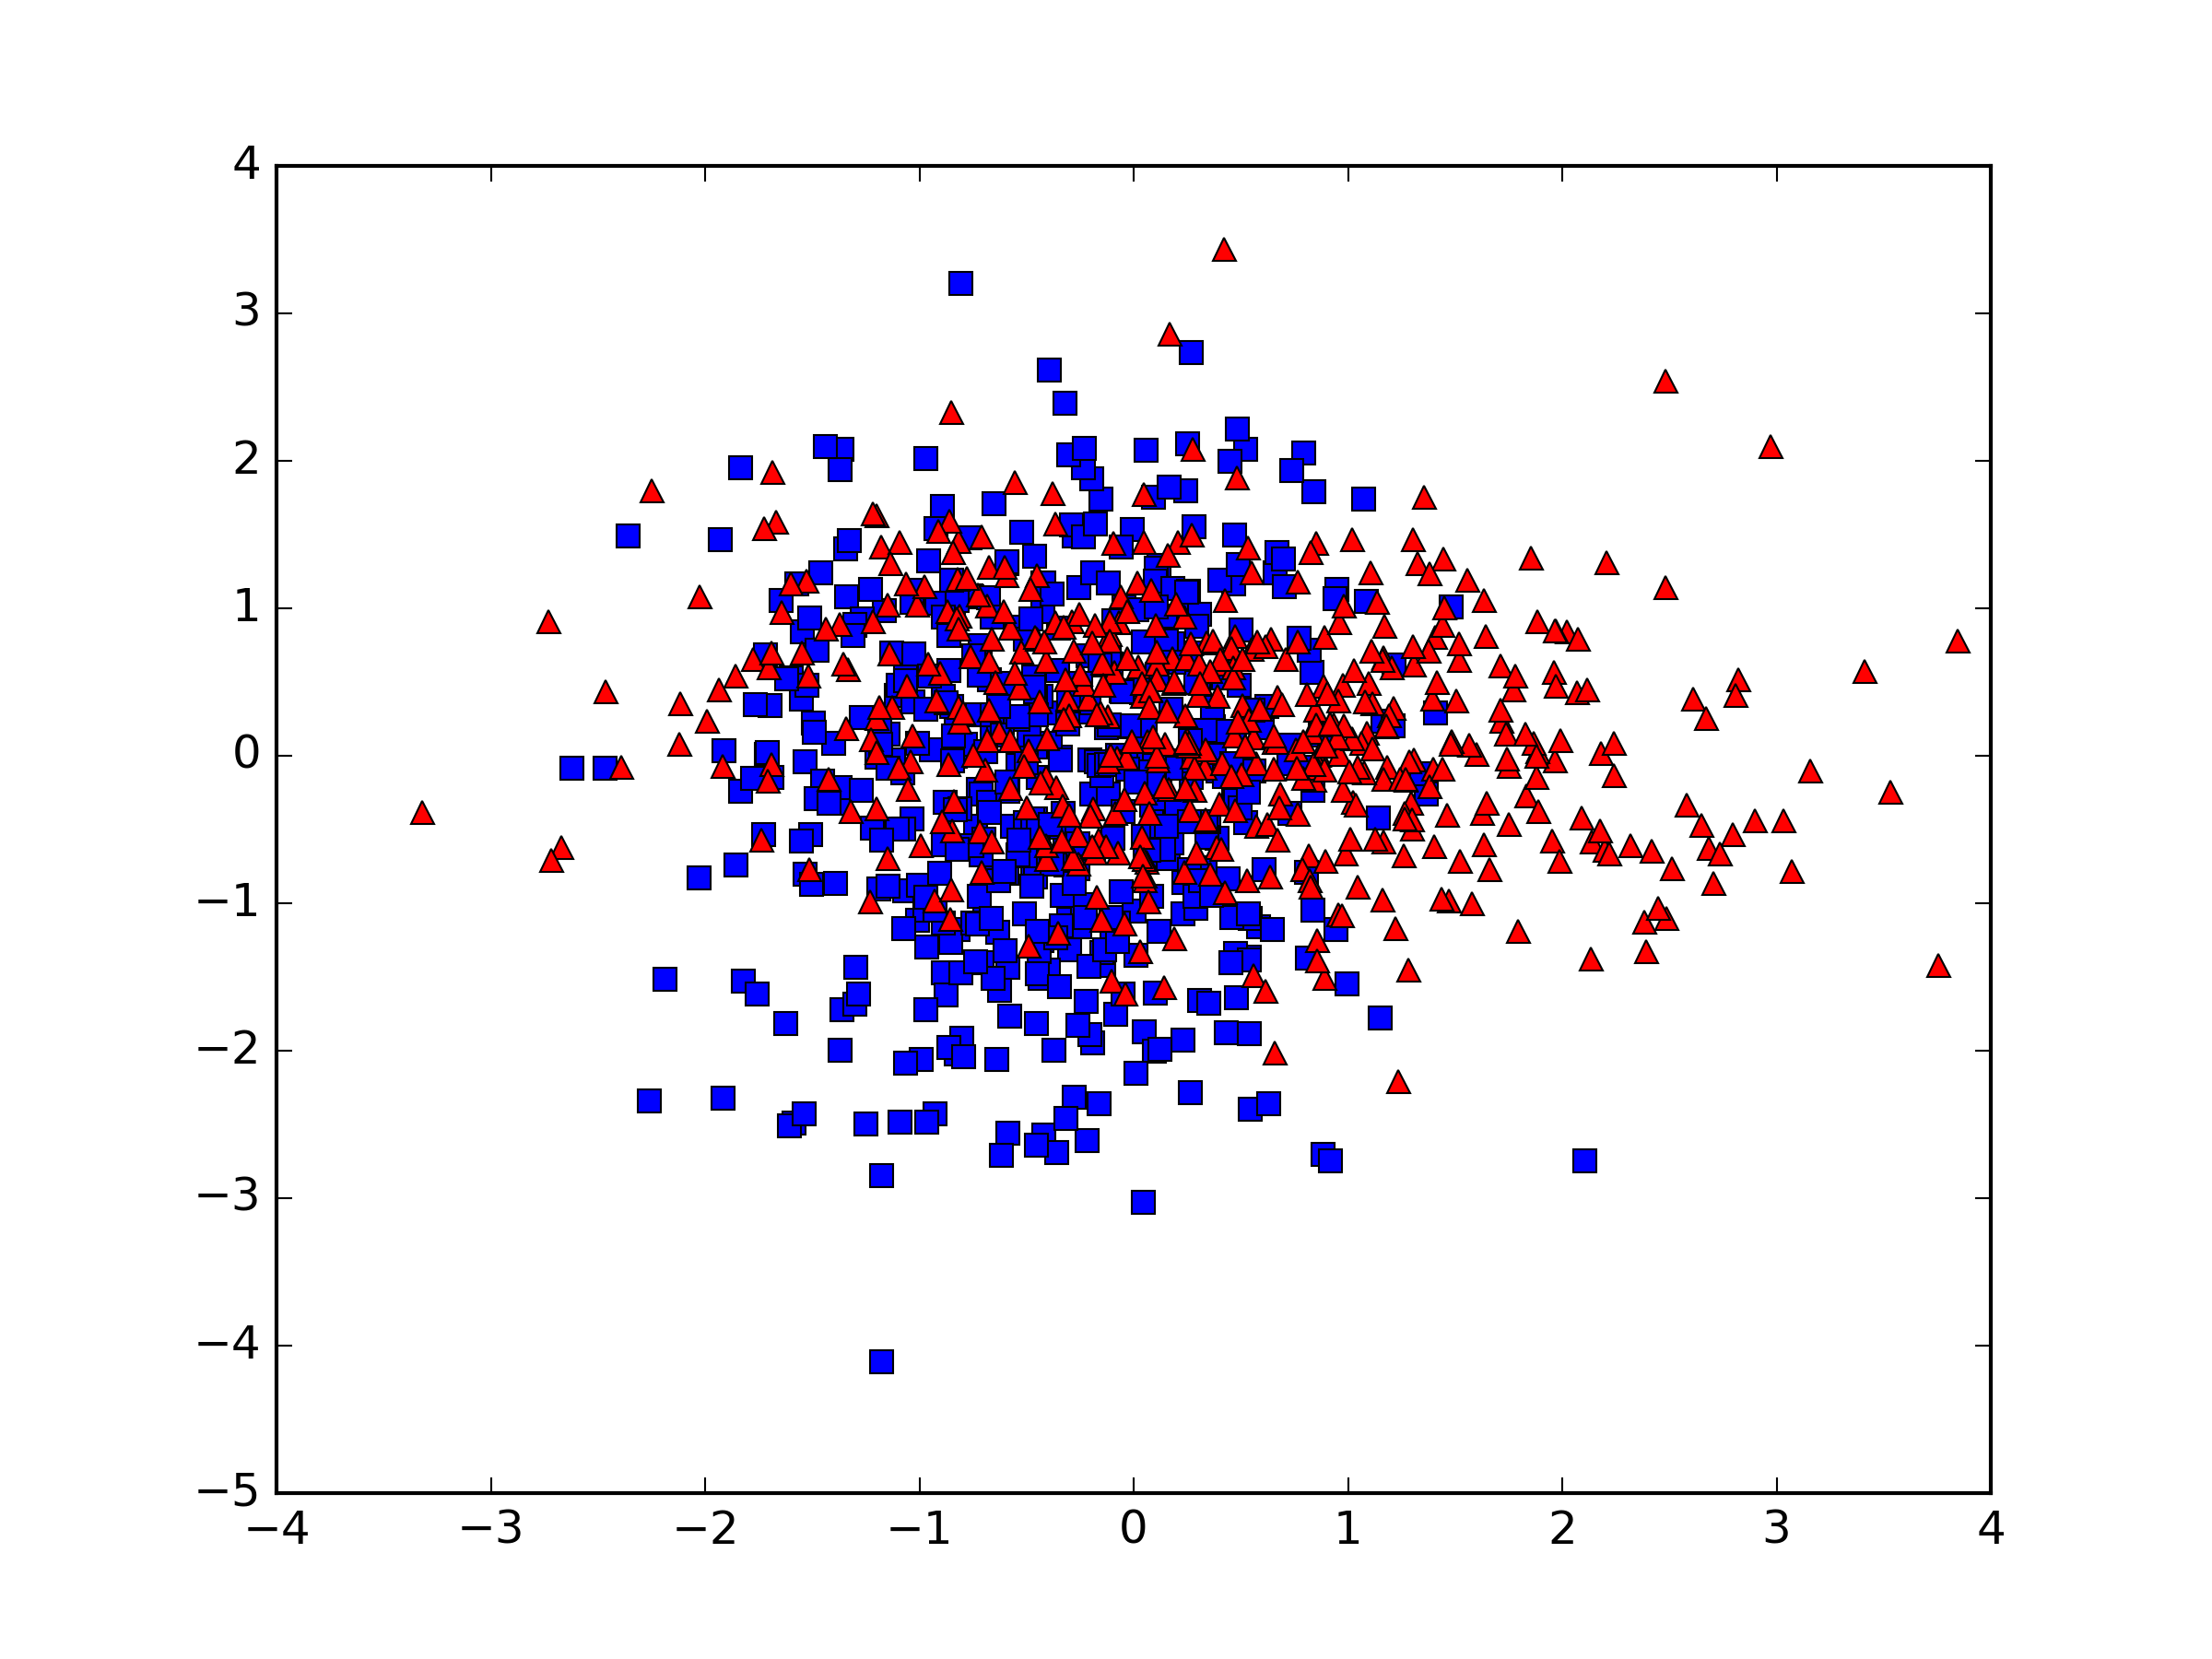
\includegraphics[scale=0.45]{img/svm_tm_n5_N131072_k3--2d_}
\end{figure}
\end{frame}

\begin{frame}{LinearSVM using RFF vs SVM. Running time}
\begin{figure}
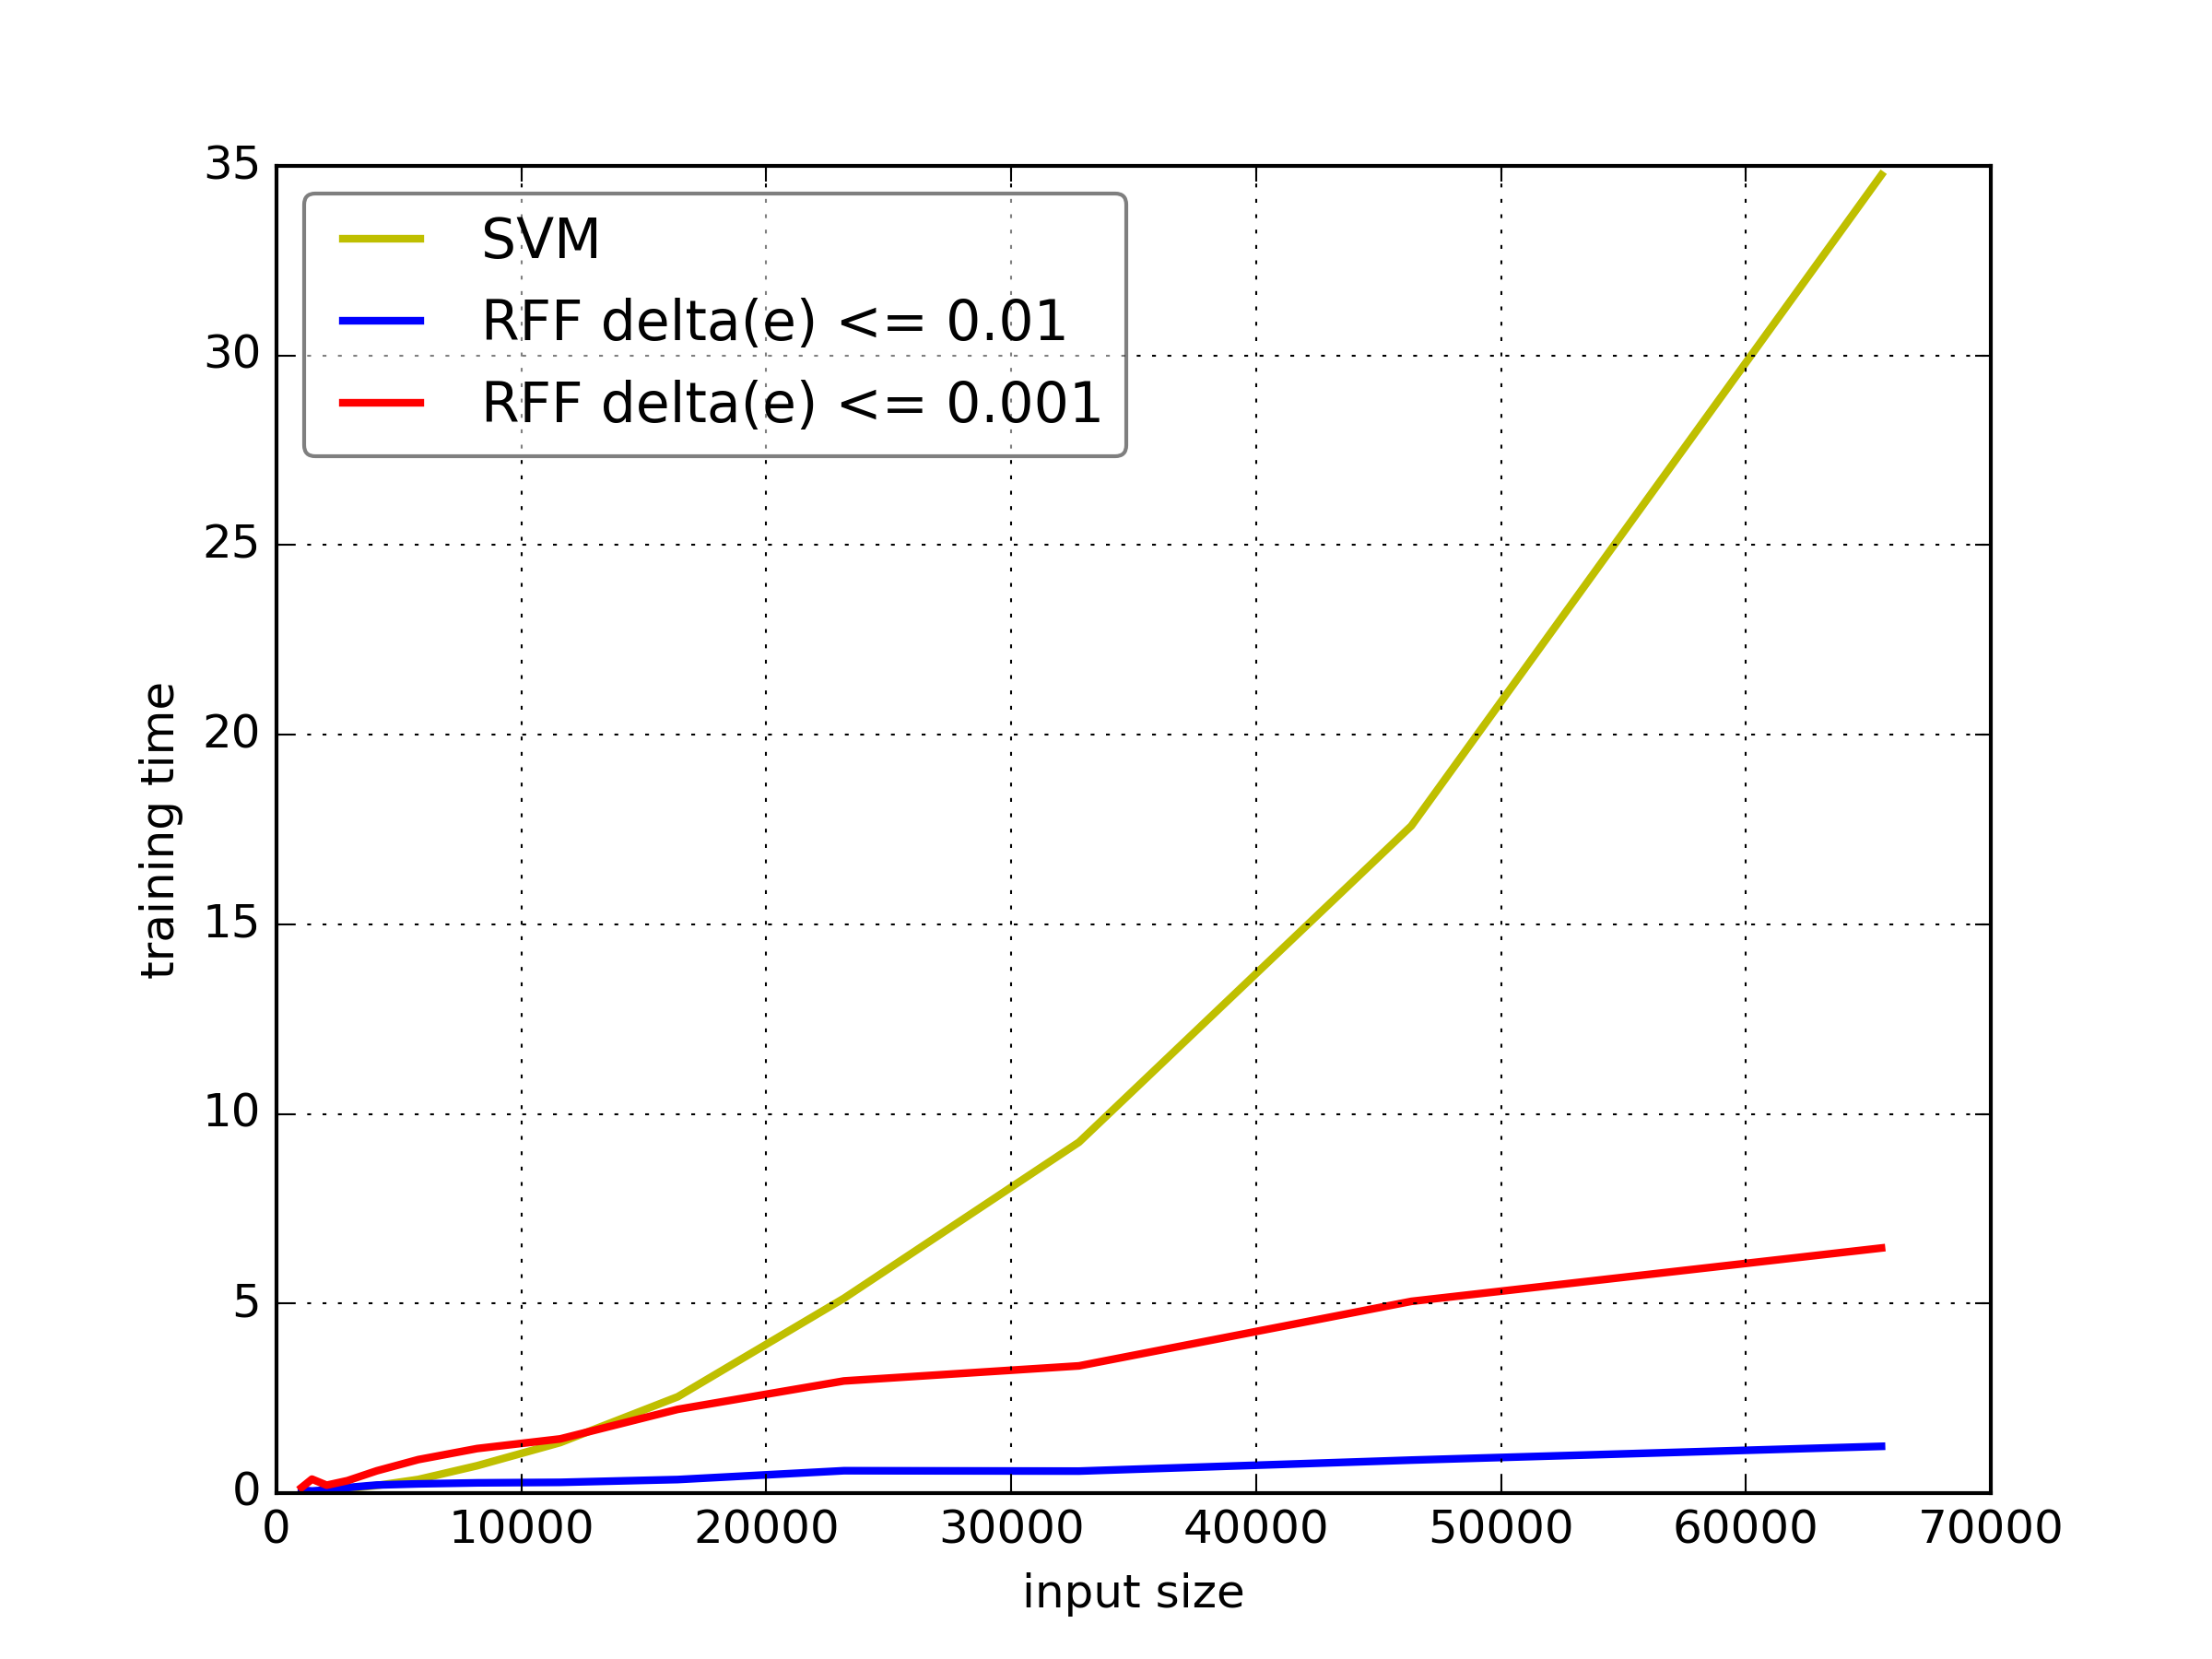
\includegraphics[scale=0.45]{img/svm_tm_n10_N131072_k10--lin_}
\end{figure}
\end{frame}

\begin{frame}[noframenumbering]{LinearSVM using RFF vs SVM. Running time}
\begin{figure}
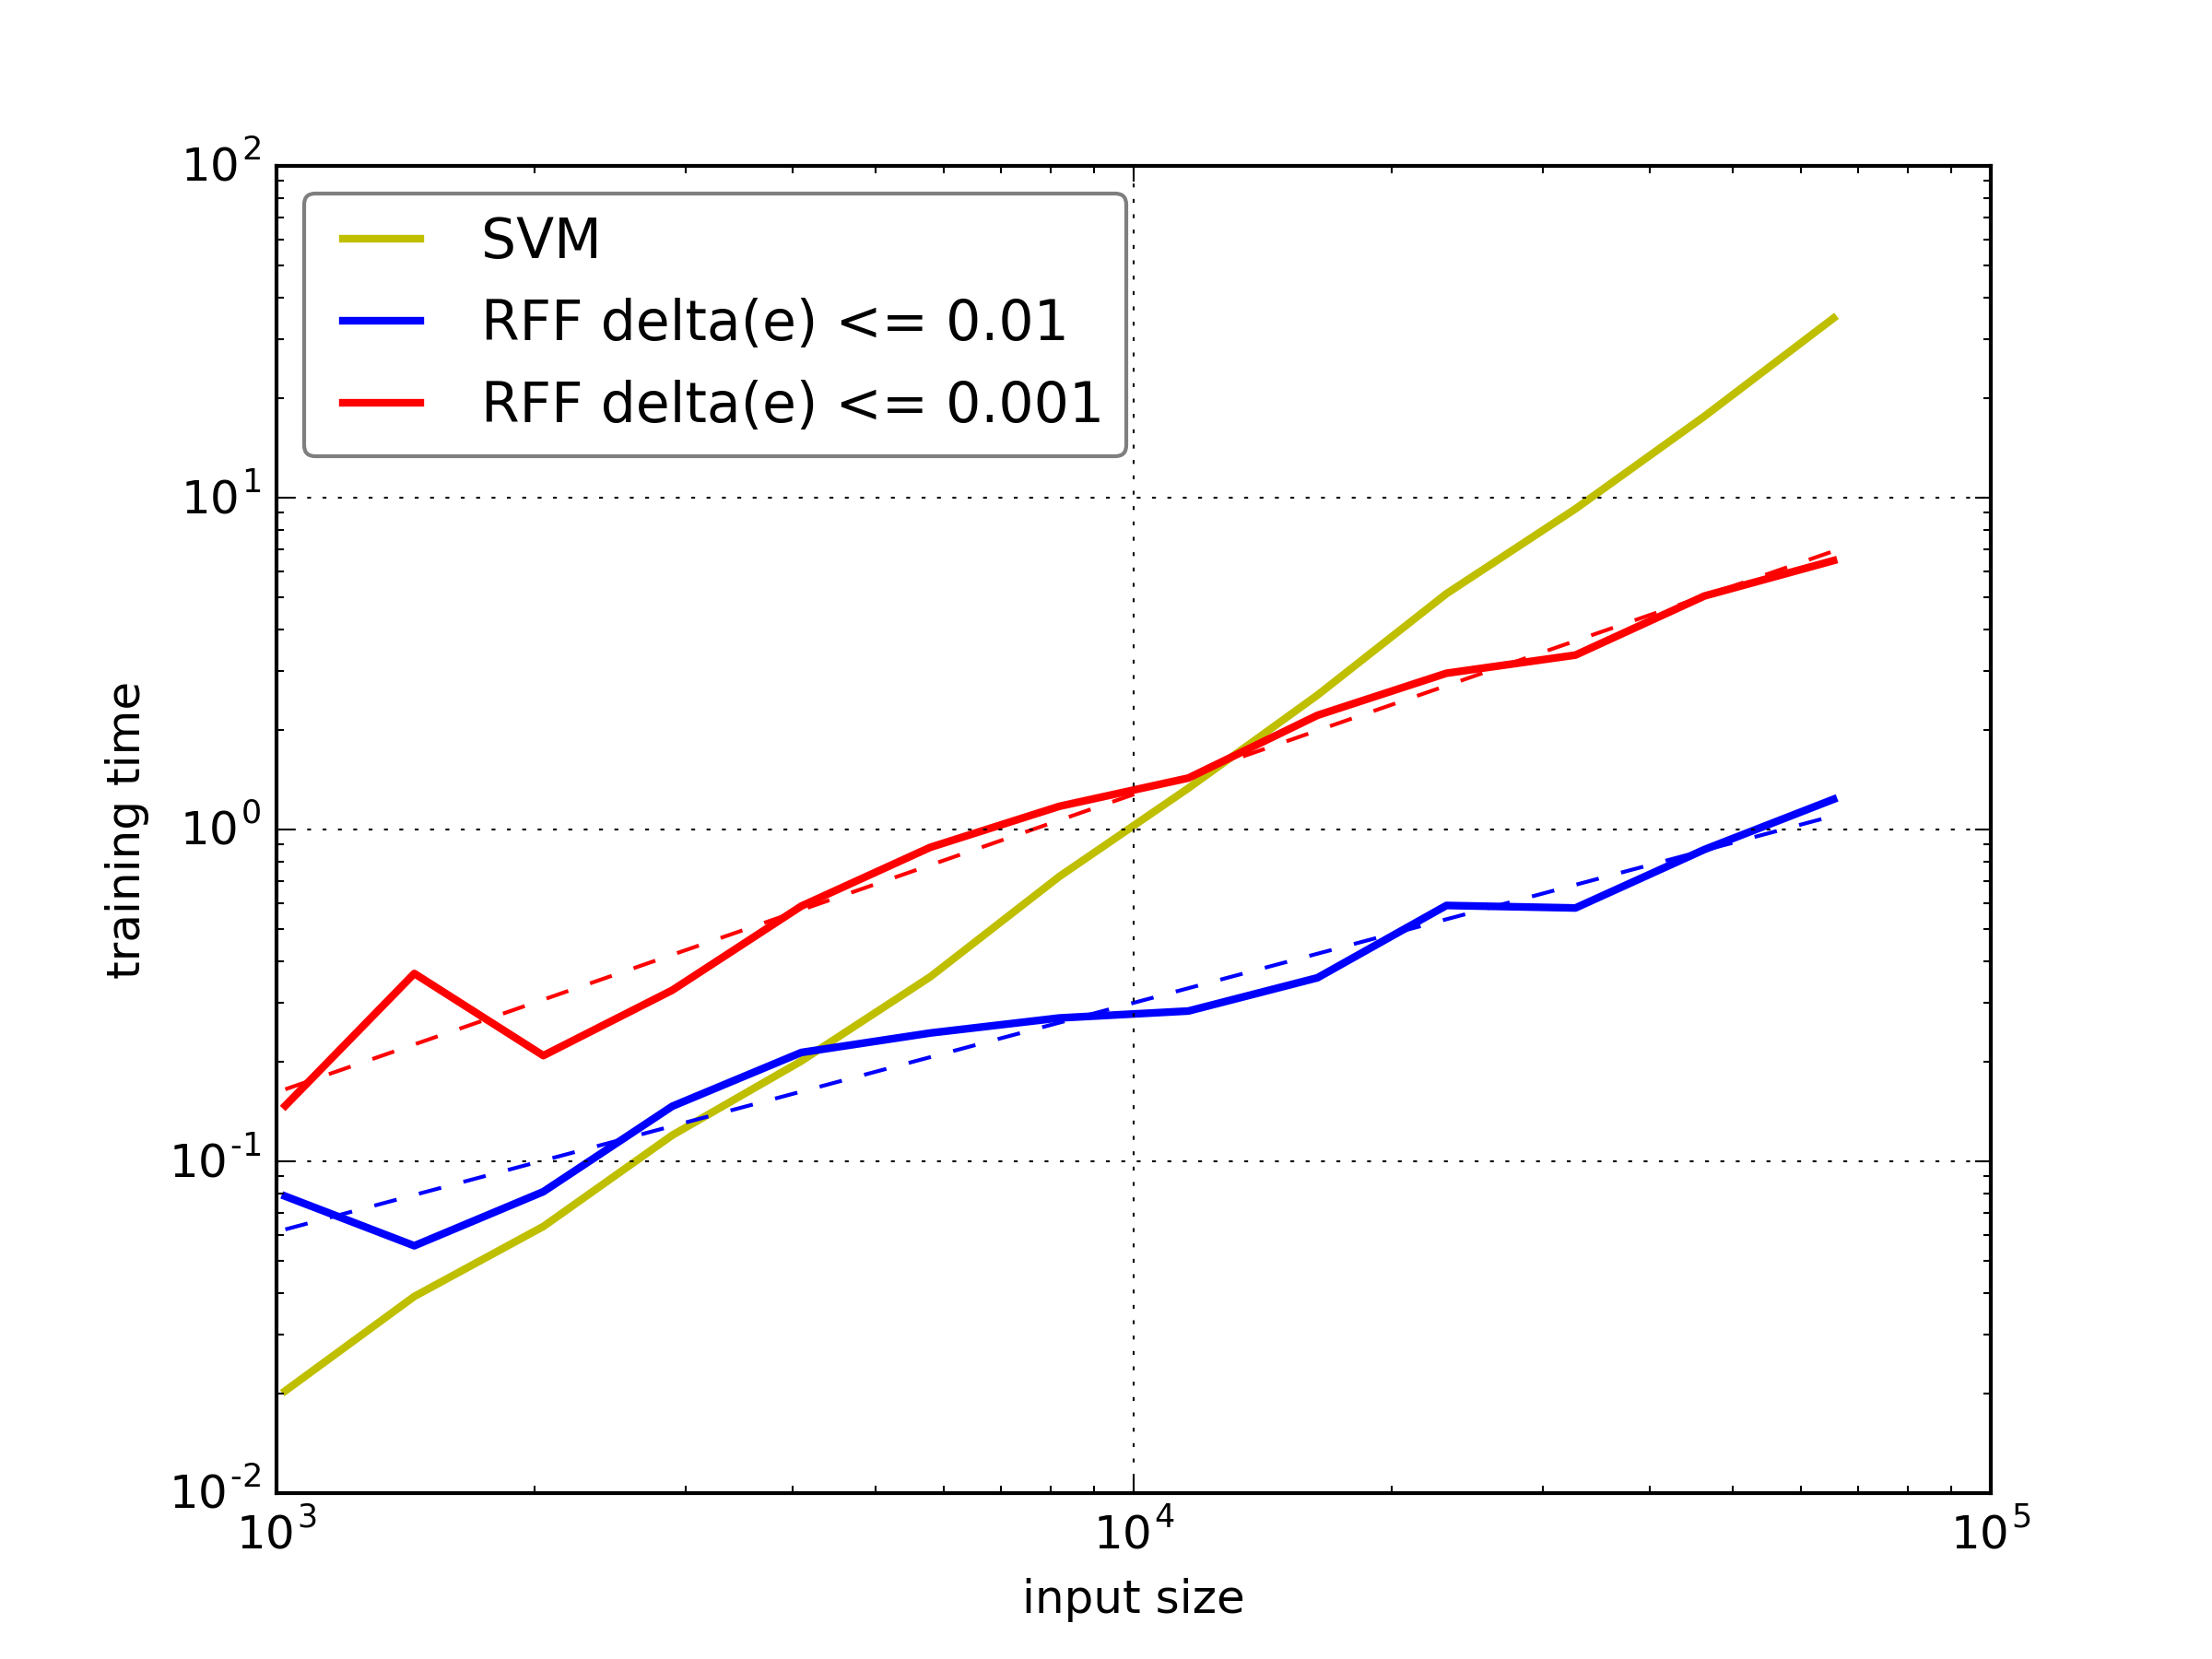
\includegraphics[scale=0.45]{img/svm_tm_n10_N131072_k10-lolo_}
\end{figure}
\end{frame}

\begin{frame}{LinearSVM using RFF vs SVM. Evaluation time}
\begin{figure}
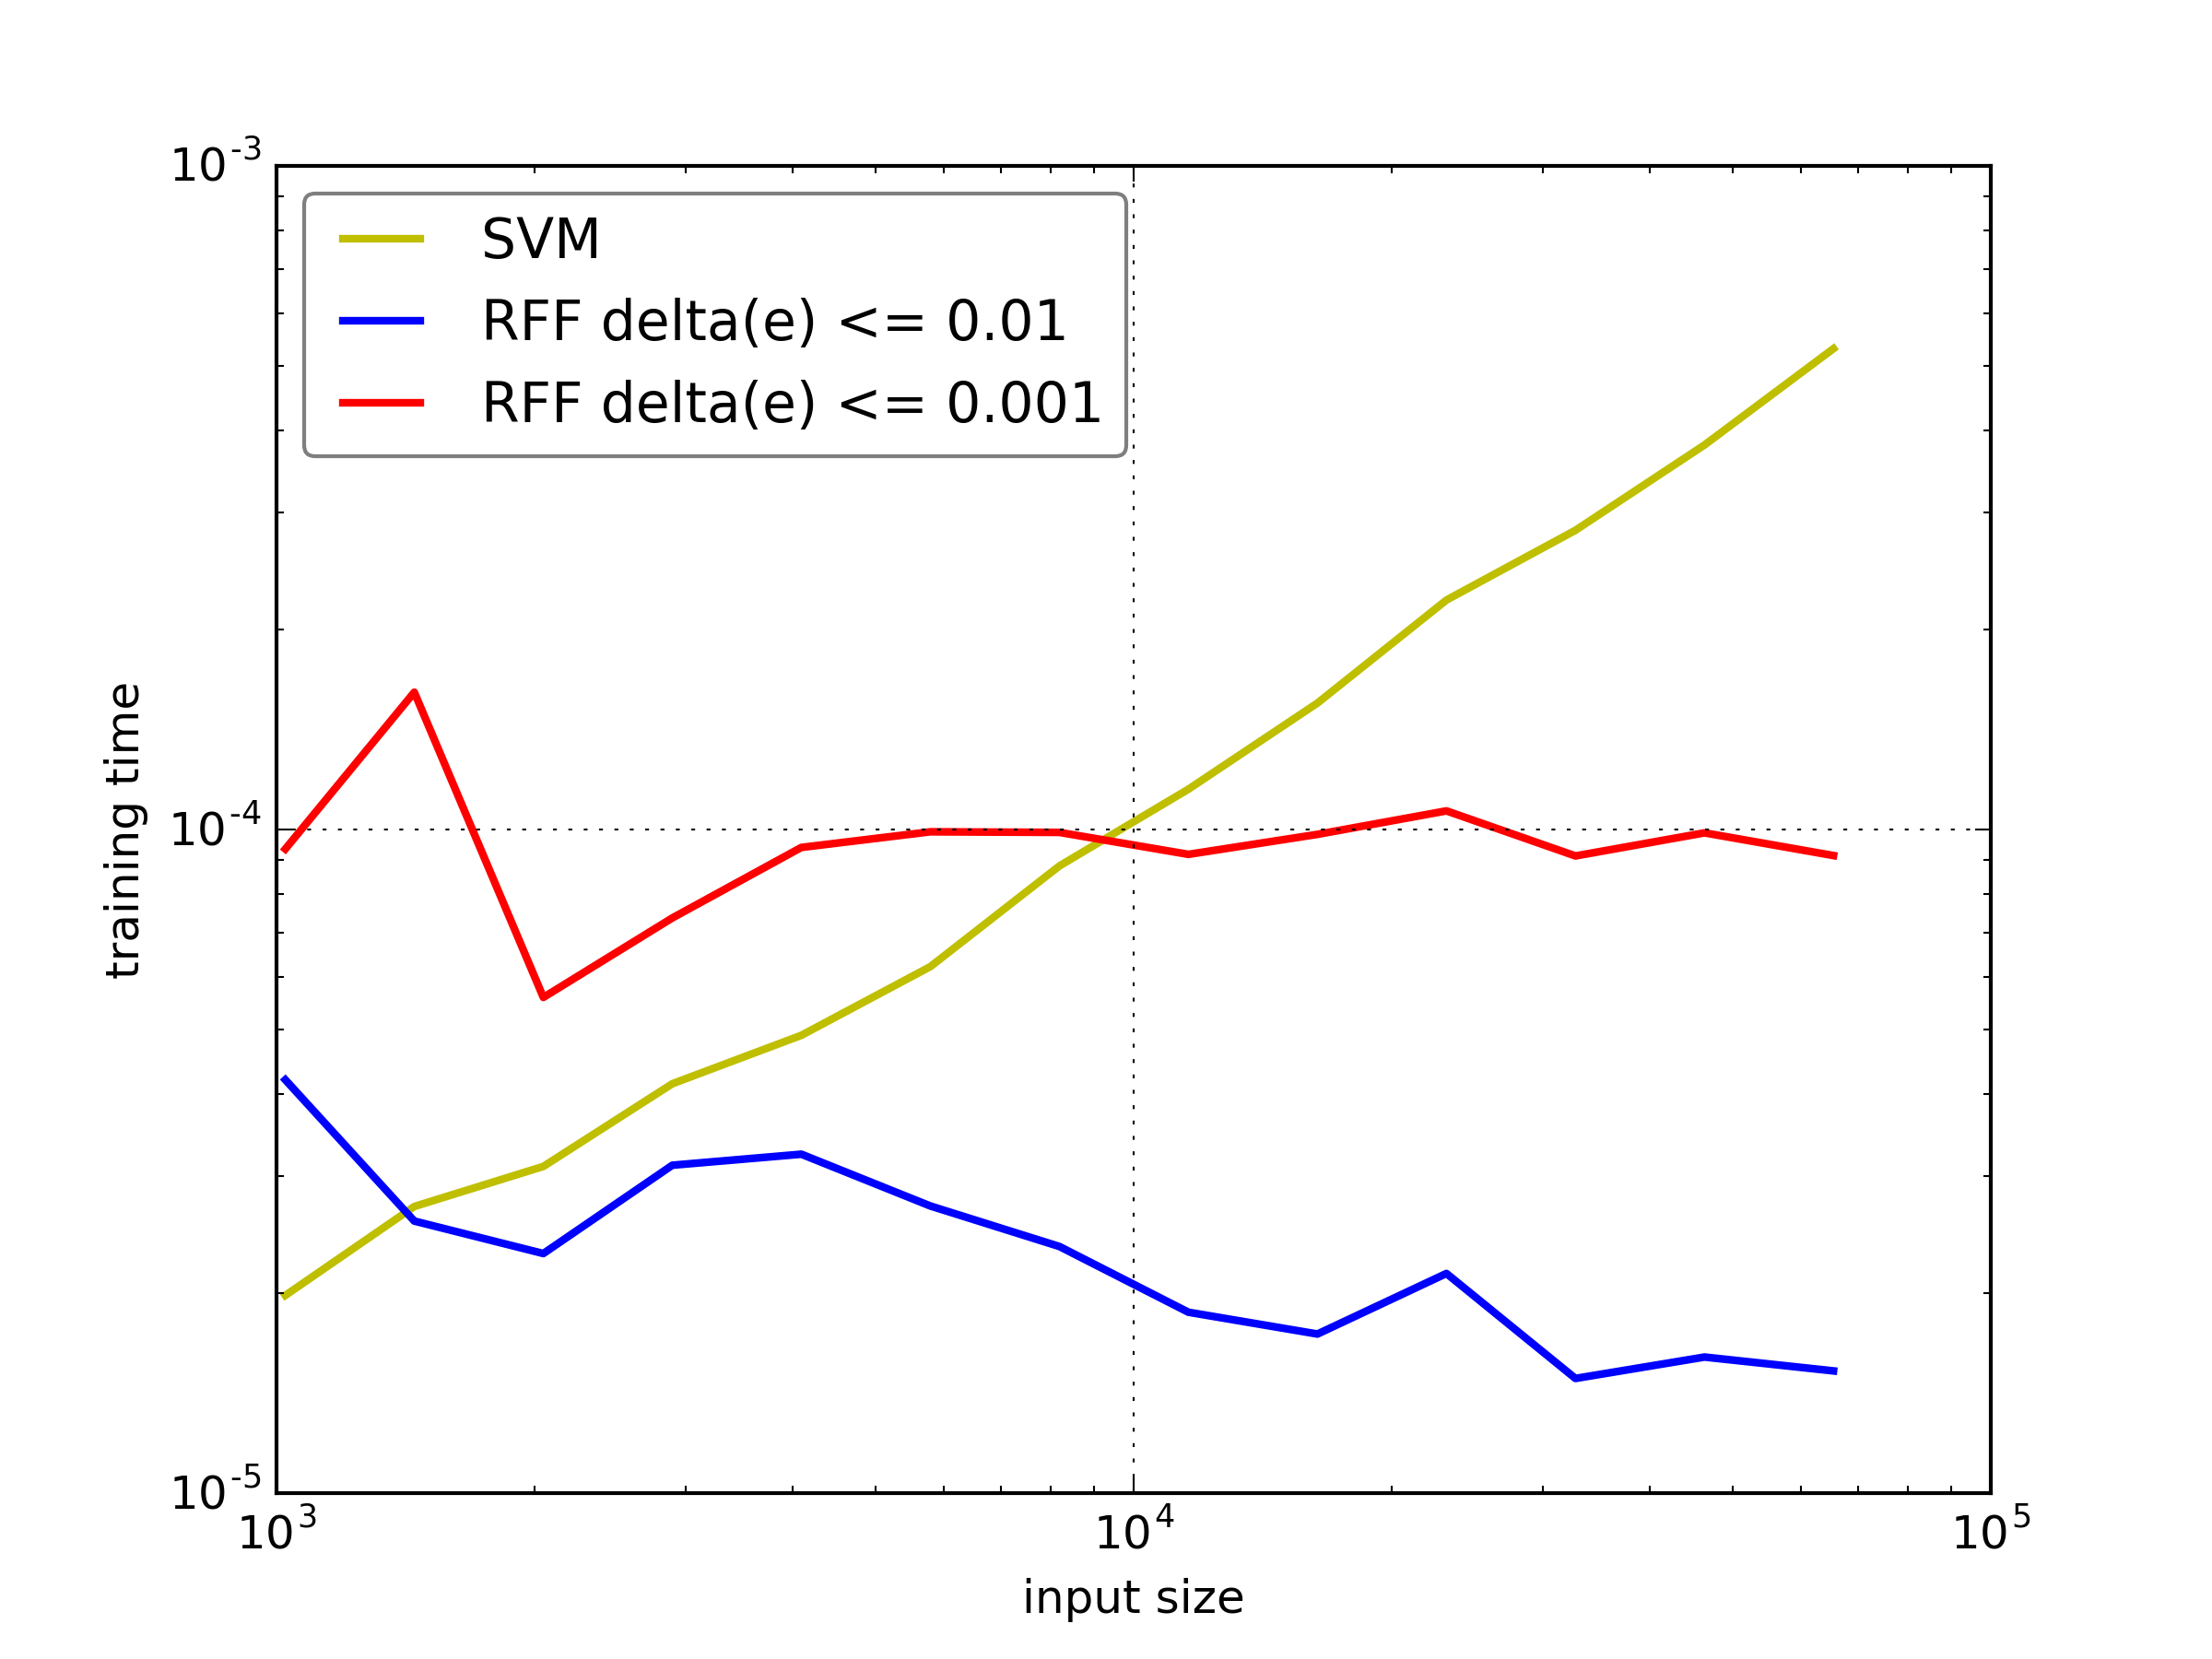
\includegraphics[scale=0.45]{img/svm_tm_n10_N131072_k10--eval_}
\end{figure}
\end{frame}

\begin{frame}{Time/Accuracy tradeoff of SVM approximation}
 D=[100, 320, 1000, 3200, 10000], N=10000
\begin{figure}
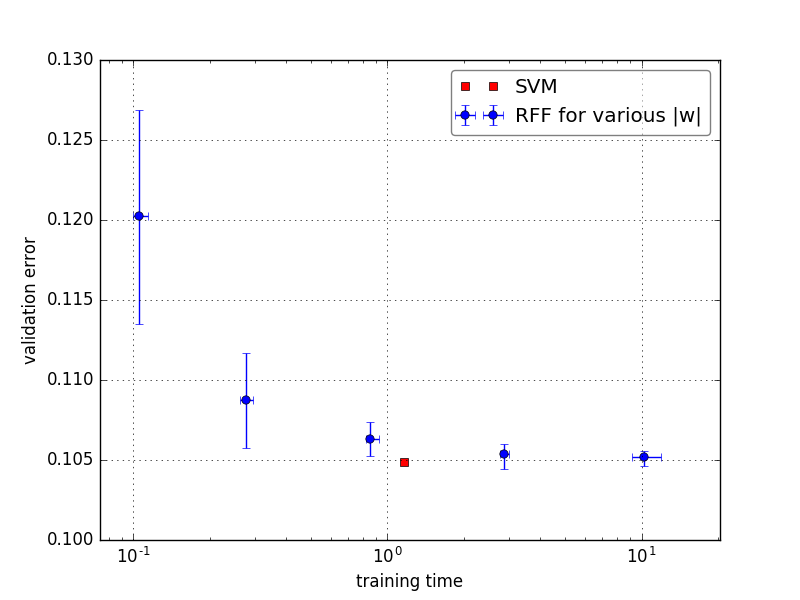
\includegraphics[scale=0.40]{img/svm_timeerror_10-90_n6N10000k50k5}
\end{figure}

\end{frame}

\begin{frame}{Conclusion}
\begin{itemize}
  \item Experimental data confirms theoretical finding by Rahimi and Recht. Some inputs show even greater approximation speed than stated in the paper
  \item Approximating linearSVM maintains linear complexity in input size for a fixed approximation error
  \item General SVM algorithm has superior accuracy and it should be chosen when possible
\end{itemize}

\end{frame}


\begin{frame}[noframenumbering]{SVM}
Primal form:
\begin{equation}
\min\limits_{\omega, b}\sum_{i=1}^n L(x_i, y_i) + \lambda ||w||^2
\end{equation}
\begin{equation}
L(x, t) \text{ - loss funciton, and } \lambda \epsilon (0, \infty)
\end{equation}
Dual form:
\begin{equation}\label{eq:dual}
\max\limits_{\alpha} \sum_{i=1}^n \alpha_i -1/2 \sum_{i,j=1}^n \alpha_i\alpha_j y_i y_j \langle x_i, x_j\rangle
\end{equation}
\begin{equation}\label{eq:dual}
\alpha_i > 0 \text{ for } \forall i \text{ and } \sum_{i=1}^n\alpha_i y_i=0
\end{equation}

\end{frame}

\begin{frame}[noframenumbering]{RFF}
\begin{equation}
\begin{aligned}
&k_s(x-y)=\int_{\mathbb{R}^d} p(\omega) e^{j\omega^T(x-y)} d\omega = \int_{\mathbb{R}^d} p(\omega) cos \omega(x-y) d\omega \\
&k_s(x-y)=E_\omega[\zeta_\omega(x)\zeta_\omega(y)^*], \text{ where } \omega \text{ are drawn from } p. \\
&k_s(x-y) =E_\omega[cos\omega(x-y)]\approx z_\omega(x)z_\omega(y)^*\\
&z_\omega(x)=\sqrt{2}cos(\omega'x+b), \text{ where } b\epsilon[0, 2\pi]
\end{aligned}
\end{equation}
\end{frame}

\end{document}
